\documentclass[12pt]{amsart}
% Default margins are too wide all the way around. I reset them here
\setlength{\hoffset}{-.75in}
\setlength{\textwidth}{6.5in}
\setlength{\voffset}{-.5in}
\setlength{\textheight}{9.0in}
\usepackage{amsmath}
\usepackage{amssymb}
\usepackage{amsthm}
\usepackage{pgfplots}
\usepackage{enumerate}
\usepackage{tikz}
\usetikzlibrary{shadows,arrows,arrows.meta,shapes,positioning,calc}% Required for the Circle and Triangle arrow tips
\usepackage{setspace}
\usepackage{siunitx}
\usepackage{enumitem}
\usepackage{tcolorbox}
\usepackage{array}
\usepackage{microtype}
\usepackage{hyperref}
\usepackage{upgreek}

\theoremstyle{conjecture}
\newtheorem{conjecture}{Conjecture}

\theoremstyle{definition}
\newtheorem{definition}{Definition}

\theoremstyle{question}
\newtheorem{question}{Question}

\theoremstyle{theorem}
\newtheorem{theorem}{Theorem}

\newenvironment{solution}
{\begin{proof}[Solution]}
{\end{proof}}

\newcommand{\sectionrule}{%
    \vspace{0.3em}
    \hrule
    \vspace{0.8em}
}

\newcommand{\vct}[1]{\underline{#1}}
\newcommand{\sys}[2]{\begin{aligned}#1\\#2\end{aligned}}
\newcommand{\rulehead}[1]{\vspace{2pt}\hrule\vspace{5pt}{\large\bfseries #1}\par}

\newcommand{\phaseplot}[1]{%
    \par\medskip
    \noindent\begin{minipage}{\linewidth}
    \centering
    \begin{tikzpicture}
    \begin{axis}[
    width=0.61\linewidth,height=4.75cm,
    axis lines=middle,
    xmin=-3.3,xmax=3.3,ymin=-1.12,ymax=1.16,
    xtick={-3,-2,-1,1,2,3},ytick={-1,-0.5,0.5,1},
    minor tick num=4,
    xlabel={$x$},ylabel={},
    title={\small functions},title style={yshift=-0.6em},
    tick label style={font=\small},
    every axis x label/.style={at={(ticklabel* cs:1)},anchor=west},
    axis line style={gray!70},tick style={gray!70},
    clip=false]
    \addplot[blue!55!gray,thick,domain=-3.3:3.3,samples=150]{sin(deg(x))};
    \addplot[orange!85!yellow!70!black,thick,domain=-3.2:3.2]{#1};
    \end{axis}
    \end{tikzpicture}
    \end{minipage}
    \par\medskip}

\title{Dynamical Systems:\\Class September 15, 2026\\ 6. 2D Nonlinear Systems and Fixed Points}
\author{Rob Tompkins}
\date{\today}


\begin{document}

    \maketitle
    {\large\bfseries Teams}

    Post screenshots of your work to the course Google Drive today: Link to drive folder. Include words, labels, and other short notes on your whiteboard that might make those solutions useful to you or your classmates. Name your images using the format:
    \begin{itemize}\item \texttt{teamXX-YY.EXT}\end{itemize}
    where XX is your two-digit team number (e.g. 06 if you are team 6), YY is the two digit number of image for today (e.g. 01 for the first image, 02 for the second, and so on.), and EXT is the extension for the image filetype you used.
    \qquad\\
    \qquad\\
    {\large\bfseries Team Activity}

    \textbf{Three ways to find a conserved quantity:}

    \begin{enumerate}

        \item Consider a system of the form $m\ddot{x}=F(x)$ where $F(x)=-\dfrac{dV}{dx}$ with $V(x)$
        called the \textbf{potential energy}. $E=\frac12 m\dot{x}^{2}+V$ is a conserved quantity for
        this system.

    \end{enumerate}

    \textbf{Example:} Let $\ddot{x}=x^3$.

    By introducing $y=\dot{x}$, this can be written as the system $\dot{x}=y,\dot{y}=x^3$. Then we have

    \[
        V(x)=-\int x^3\,dx=-x^4/4.
    \]

    Try $E=\frac12 y^2-x^4/4$. Is this conserved? (It should be).

    \[
        \frac{dE}{dt}=y\dot{y}-x^3\dot{x}=yx^3-x^3y=0.
    \]

    It is conserved!

    \begin{center}
        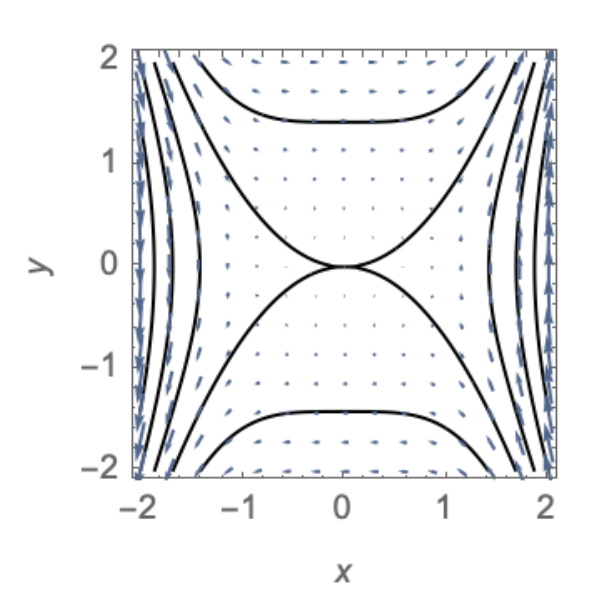
\includegraphics[width=0.3\linewidth]{figures/quartic-phase.png}
    \end{center}

    \textbf{Problem 1:} Let $\ddot{x}=-kx$. Find $E$ and check that it is conserved.

    \begin{enumerate}[start=2]

\item A \textbf{phase curve} of a system $\dot{x}=f(x,y),\dot{y}=g(x,y)$ is a curve $y=Y(x)$
(note that $\dot{y}=Y_x\dot{x}$) that obeys the differential equation
$\frac{dY}{dx}=\frac{\dot{y}}{\dot{x}}=\frac{g(x,Y)}{f(x,Y)}$. Trajectories that start on such
a curve stay on it. When $\frac{dy}{dx}=\frac{g(x,y)}{f(x,y)}$ is a separable differential
equation, the process of solving it can also yield a conserved quantity.

    \end{enumerate}

    \textbf{Problem 2:} A model of two species with exponential population growth and competition
    is given by

    \[
        \begin{aligned}
            N_1'&=r_1N_1-\alpha_1N_1N_2\\
            N_2'&=r_2N_2-\alpha_2N_1N_2.
        \end{aligned}
    \]

    The model nondimensionalizes to

    \[
        \begin{aligned}
            x'&=x-xy\\
            y'&=y(\rho-x).
        \end{aligned}
    \]

    This nondimensionalization requires assuming that each population has its own units, so number
    of rabbits and number of sheep were each be assigned their own unknown constant in the
    nondimensionalization process.

    \begin{itemize}

        \item Using the nondimensional system, find an expression satisfied by most phase curves. Solve
        a separable differential equation to do this. You don't need to write it in the form $y=Y(x)$;
        an implicit relationship between $x$ and $y$ is fine.

        \item Argue that the quantity $H(x,y)=y-\ln y+\rho\ln x-x$ is almost always conserved.

        Which trajectories don't work with this function?

    \end{itemize}

    \begin{center}
        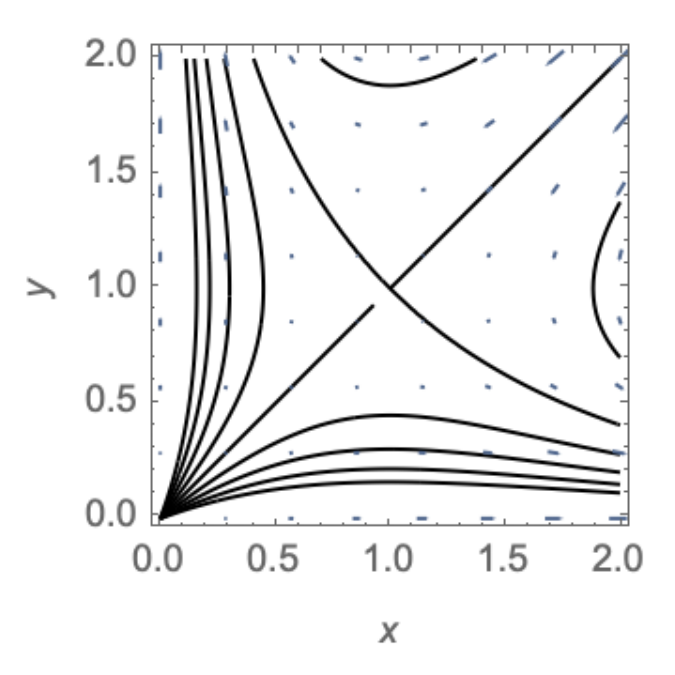
\includegraphics[width=0.34\linewidth]{figures/competition-phase.png}
    \end{center}

    \begin{enumerate}[start=3]

\item A \textbf{Hamiltonian function}, $H(x,y)$ is an energy function. The associated dynamical
system $\dot{x}=\frac{\partial H}{\partial y}$, $\dot{y}=-\frac{\partial H}{\partial x}$ is
called a \textbf{Hamiltonian system}. In a Hamiltonian system, the Hamiltonian is a conserved
quantity.

    \end{enumerate}

    \textbf{Problem 3:} Let $\dot{x}=x^2,\dot{y}=-2xy+x$. Show this system is Hamiltonian.

    \textbf{Problem 4:} Consider the system

    \[
        \begin{aligned}
            \dot{x}&=-\mu y+xy\\
            \dot{y}&=\mu x+\frac12(x^2-y^2).
        \end{aligned}
    \]

    Assume $\mu>0$.

    \begin{enumerate}[label=(\alph*)]

\item This system has a conserved quantity. Assume $\dot{x}=H_y$ and $\dot{y}=-H_x$ for an
unknown function $H(x,y)$. If our assumption is correct then
$\partial_x\dot{x}=-\partial_y\dot{y}$. Why is that?

\item Show that $\partial_x\dot{x}=-\partial_y\dot{y}$ for this system.

\item Construct a function $H(x,y)$ that is conserved for this system.

\item If time permits, begin the process of constructing a phase portrait for this system.

    \end{enumerate}

    \section*{Reversible Systems:}

    A system of the form

    \[
        \begin{aligned}
            \dot{x}&=f(x,y)\\
            \dot{y}&=g(x,y)
        \end{aligned}
    \]

    is \textbf{reversible} if the change of variables $t\mapsto-t$ and $(x,y)\mapsto R(x,y)$ with
    $R^2(x,y)=(x,y)$ yields the same system, i.e. the system is invariant to this change of
    variables.

    \begin{itemize}

        \item examples of $R$: $R(x,y)=(x,-y)$ (mechanical systems, $m\ddot{x}=F(x)$) or
        $R(x,y)=(-x,-y)$. In 2D, a reflection about any axis through the origin has this property.

        \item e.g. if $f$ is odd in $y$ ($f(x,-y)=-f(x,y)$) and $g$ is even in $y$ ($g(x,-y)=g(x,y)$)

        \item Reversible systems are ``ideal'' in the sense that no energy is ``wasted.''

        \item Real systems are characterized by friction, turbulence, unrestrained expansion,
        temperature gradients and mixing of dissimilar substances and are therefore irreversible.

        \item Similar to conservative systems, but not the same thing, e.g.

        \[
            \dot{x}=y,\quad \dot{y}=x^3
        \]

        is both conservative and reversible but

        \[
            \dot{x}=-2\cos x-\cos y,\quad\dot{y}=-2\cos y-\cos x
        \]

        is only reversible. (How can you tell it is not conservative from the phase portrait below?)

    \end{itemize}

    \begin{center}
        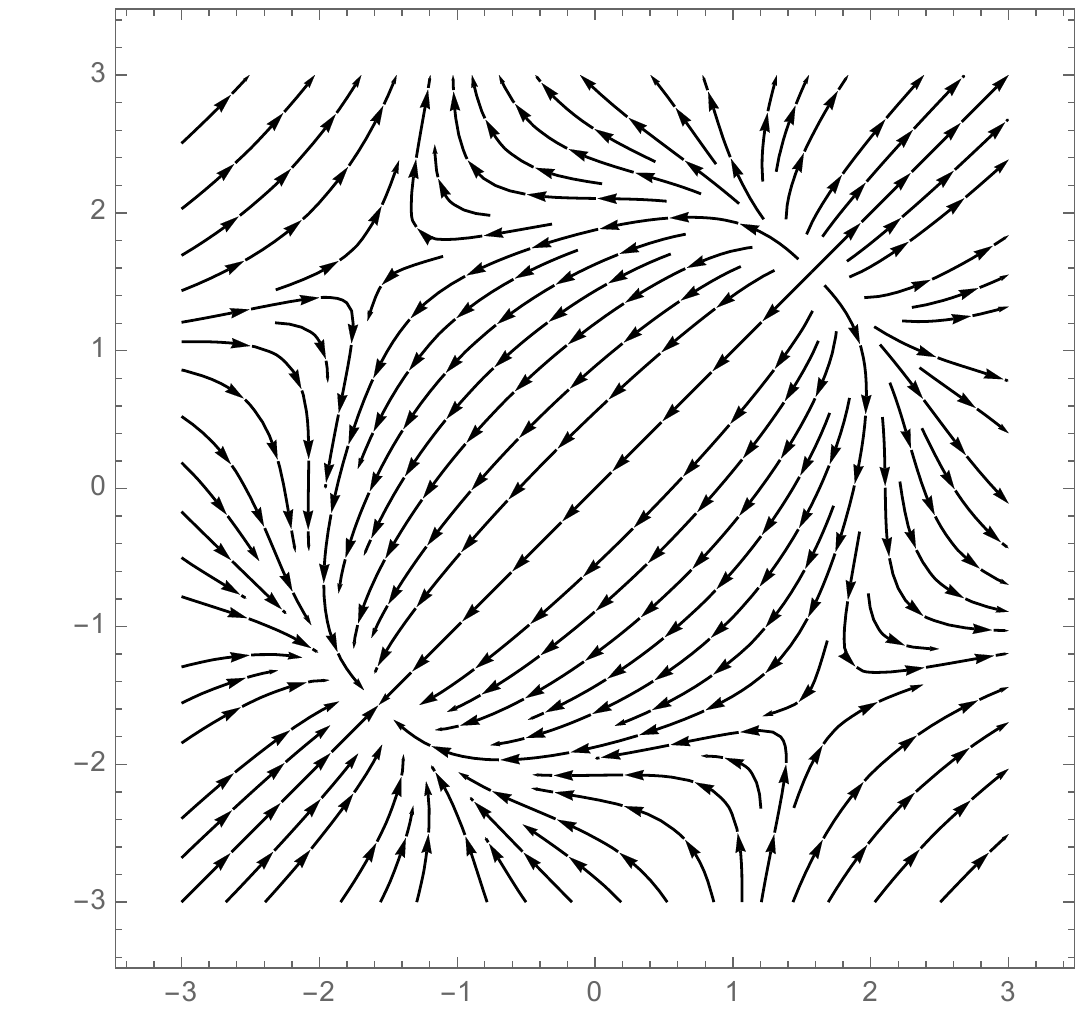
\includegraphics[width=0.54\linewidth]{figures/reversible-phase.png}
    \end{center}

    A \textbf{cylindrical phase space} arises when one coordinate can take on any value in $\mathbb
    R$ (the real numbers) while the other coordinate is an angle.

    A \textbf{toroidal phase space} arises when two coordinates are angles.

    \begin{center}
        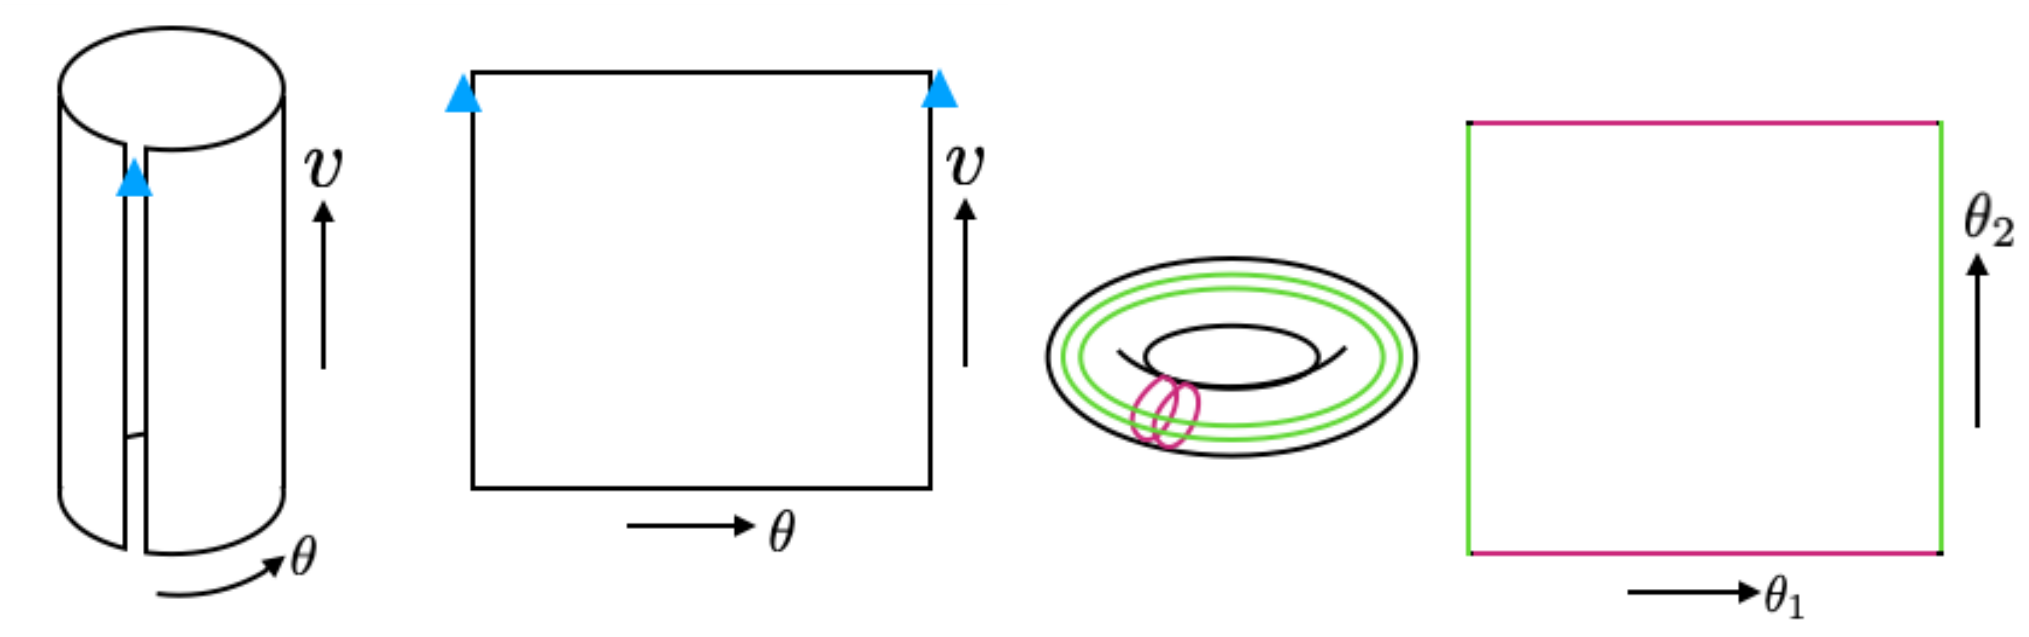
\includegraphics[width=\linewidth]{figures/cylinder-torus.png}
    \end{center}

    \textbf{Problem 5:} To get used to a phase space that is a torus, think about two oscillators
    that are not interacting (like the hour hand and the minute hand on a clock: they each go at
    their own pace, and that pace is constant).

    \begin{enumerate}[label=(\alph*)]

\item Let $\dot{\theta}_1=1$ and $\dot{\theta}_2=2$. If the oscillators each start at a phase
angle of zero, so at the point $(0,0)$, draw their trajectory onto the phase space. Use a
square to represent the space. Will the pair of oscillators pass through $(0,0)$ at some point?

\item Now let $\dot{\theta}_1=\pi$ and $\dot{\theta}_2=2\pi$. With an initial condition of
$(0,0)$, draw their trajectory onto the phase space. How is the trajectory different from the
one in part a?

\item Let $\dot{\theta}_1=\pi$ and $\dot{\theta}_2=\sqrt{2}\pi$. Assume the oscillator pair
again starts at $(0,0)$. The first oscillator will return to a phase of zero at time 2, time 4,
etc. When does the second oscillator return to a phase of zero? Will the pair pass through
$(0,0)$ at some point?

    \end{enumerate}

    \clearpage
    \section*{Answers}

    1) Potential energy practice: $\dot{x}=y,\dot{y}=-kx$. $V(x)=-\int-kx\,dx=kx^2/2$. Try
    $E=\frac12y^2+kx^2/2$. $\dot{E}=y\dot{y}+kx\dot{x}=y(-kx)+kxy=0$.

    3) Hamiltonian example: Assume $H_y=x^2$, so $H=x^2y+g(x)$ where $g(x)$ is unconstrained by $H_y$.

    Using this $H$, compute $H_x$ to find $H_x=2xy+g'(x)$. We want $-\dot{y}=H_x$, so
    $-2xy+x=-2xy-g'(x)$. This implies that $g'(x)=-x$, so $g(x)=-x^2/2+c$. We can choose $c=0$ for
    simplicity.

    So we have $H(x,y)=x^2y-x^2/2$ as a conserved quantity.

    \begin{center}
        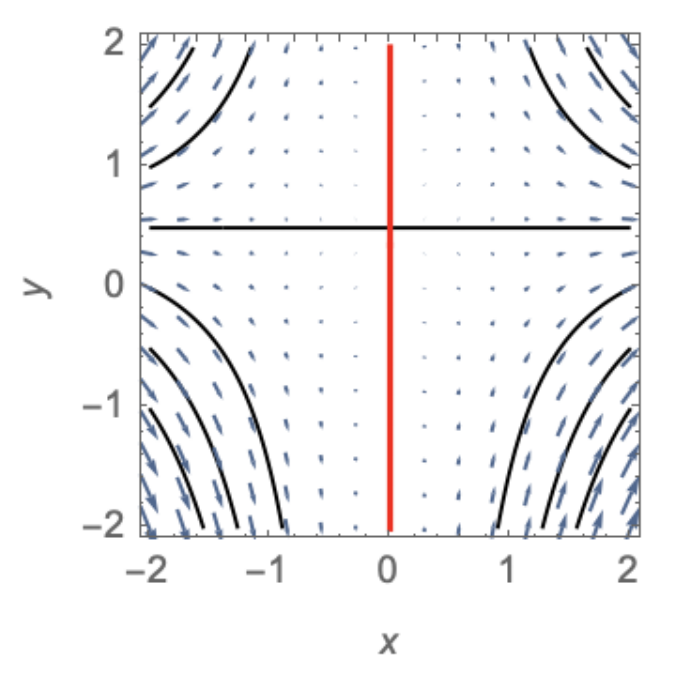
\includegraphics[width=0.34\linewidth]{figures/hamiltonian-phase.png}
    \end{center}

    4) Hamiltonian practice: a: Mixed partials are equal, $H_{xy}=H_{yx}$, so if $\dot{x}$ and
    $\dot{y}$ are given by those partials, then we can use $\dot{x}$ and $\dot{y}$ to compute the
    mixed partials in two different ways.

    b: $\partial_x\dot{x}=y$. $-\partial_y\dot{y}=-\frac12(-2y)=y$. These are equal.

    c: $H_y=-\mu y+xy$ so $H(x,y)=\frac12y^2(-\mu+x)+G(x)$. $-H_x=-\frac12y^2-G_x=\mu
    x+\frac12(x^2-y^2)$ so $G_x=-\mu x-\frac12x^2$. $G(x)=-\mu\frac12x^2-\frac16x^3+c$. I just need
    a single function that works, not a whole family of them.
    $H(x,y)=-\mu\frac12x^2-\frac16x^3+\frac12y^2(-\mu+x)$ is one such function.

    5a: (see below left) $\theta_1$ moves 1 unit in the time $\theta_2$ moves two units, so the
    trajectory is a line with slope 2 through $(0,0)$. It will leave at the top (at $(\pi,2\pi)$)
    and come back in at the bottom (at $(\pi,0)$).

    \begin{center}
        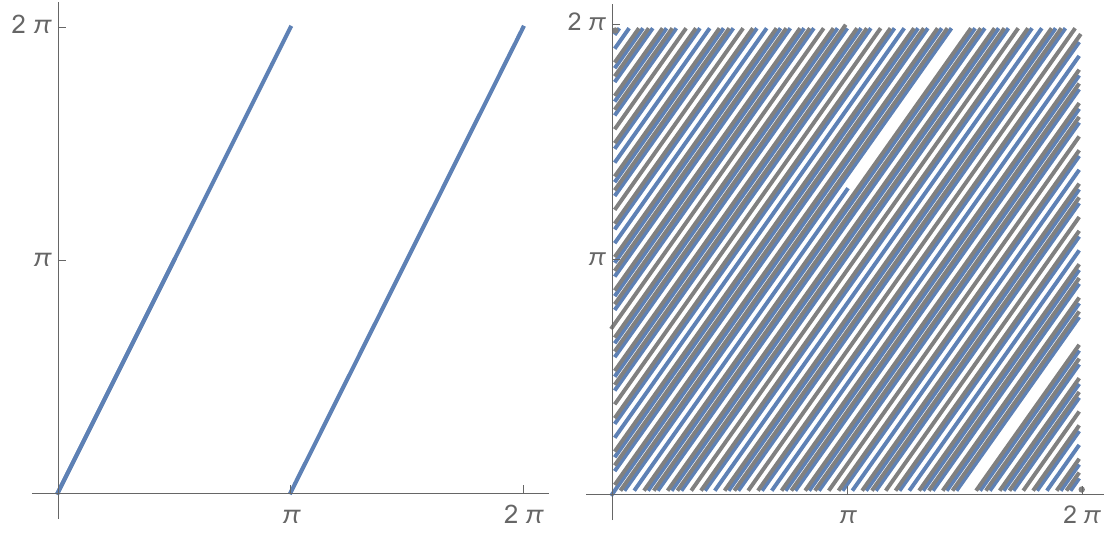
\includegraphics[width=0.55\linewidth]{figures/torus-trajectories.png}
    \end{center}

    5b: This trajectory will look the same as above. We're just moving faster along the same path.

    5c: (see above right) oscillator 1 returns to phase 0 at time 2, 4, etc, so times
    $2\mathbb{Z}^+$. oscillator 2 returns to a phase of 0 when $\sqrt{2}\pi t=2n\pi$ for $n$ an
    integer $\Rightarrow\sqrt{2}t=2n$ or when $t=\sqrt{2}n$. The return times are not integers. The
    pair of oscillators will not both return to zero at the same time, so this trajectory does not
    pass through $(0,0)$ again!

\end{document}